\section{变温间歇釜式反应器}


\begin{frame}
    \frametitle{变温操作}

    \large 研究变温操作具有很大的实际意义
    \begin{itemize}
        \item[\bullet] 对于间歇釜式反应器要做到绝对等温是极其困难的。
        \item[\bullet] 对于许多化学反应，等温操作的效果不如变温操作好。
    \end{itemize}
    
    对间歇反应器而言，确定反应过程的温度与时间的关系十分必要
    \begin{itemize}
        \item[\bullet] 温度是影响反应器操作的敏感因素，它对转化率、收率、反应速率以及反应器的生产强度都有影响。
        \item[\bullet] 温度不同，反应物系的物理性质也不同，从而影响到传热和传质速率及搅拌器的功率。
    \end{itemize}

\end{frame}


\begin{frame}
    \frametitle{反应过程能量变化}

    \large 间歇反应过程温度与时间的关系可由能量守恒定律来确定。由于间歇釜式反应器是一封闭物系，如果不考虑搅拌器对反应物系所作的功，则由热力学第一定律可得
    \[
        \dif q = \dif U
    \]
    即反应物系与环境交换的热量等于内能的变化。
    
    事实上反应器中物料的内能变化和焓变$\dif H$并无显著差别，特别是液相物系，所以，为了计算方便和实用的目的，用下式来代替
    \[
        \dif q = \dif H
    \]
    时间间隔$\dif t$内，反应物系与环境交换的热量 = 焓变

\end{frame}



\begin{frame}
    \frametitle{$\dif H$的计算}
    \begin{center}
        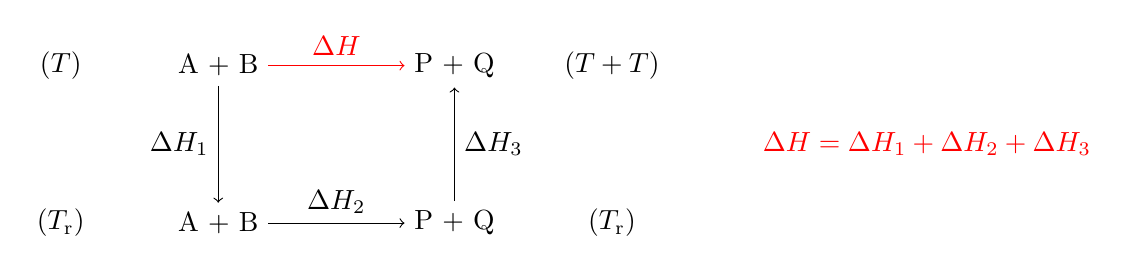
\begin{tikzpicture}
            \node (A) at (0,0) {$(T_\mathrm{r})$};
            \node (B) at (2,0) {A + B};
            \node (C) at (5,0) {P + Q};
            \node (D) at (7,0) {$(T_\mathrm{r})$};
            \node (a) at (0,2) {$(T)$};
            \node (b) at (2,2) {A + B};
            \node (c) at (5,2) {P + Q};
            \node (d) at (7,2) {$(T + \dif T)$};
            \draw [->] (b) -- (B) node[left,midway]{$\Delta H_1$};
            \draw [->] (B) -- (C) node[above,midway]{$\Delta H_2$};
            \draw [->] (C) -- (c) node[right,midway]{$\Delta H_3$};
            \draw [->,red] (b) -- (c) node[above,midway]{$\Delta H$};
            \node [red] at (11,1) {$\Delta  H = \Delta H_{1}+\Delta  H_{2}+\Delta H_{3}$};
            \end{tikzpicture}
    \end{center}

    \begin{align*}
        \Delta H_{1}&=m_{\mathrm{t}} \int_{T}^{T_{\mathrm{r}}} C_{\mathrm{pt}} \dif  T \approx m_{\mathrm{t}} \bar{C}_{\mathrm{pt}}(T_{\mathrm{r}}-T)  \\
        \Delta  H_{2} &= \Delta H_{\mathrm{r}}(-\mathscr{R}_{\mathrm{A}}) V_{\mathrm{r}} \dif  t \\
        \Delta H_{3} &\approx m_{\mathrm{t}} \bar{C}_{\mathrm{pt}}(T+\dif  T-T_{\mathrm{r}}) \\
        \Delta  H &= \Delta H_{1}+\Delta  H_{2}+\Delta H_{3}=m_{\mathrm{t}} \bar{C}_{\mathrm{pt}} \dif  T+\Delta H_{r}(-\mathscr{R}_{\mathrm{A}}) V_{\mathrm{r}} \dif  t 
      \end{align*}
    

\end{frame}



\begin{frame}
    \frametitle{与环境交换的热量}

    \large 反应物系与环境交换的热量为
    \[
        \dif q = UA_\mathrm{h}(T_\mathrm{c}-T)\dif t
    \]
    式中，$U$为总传热系数；$A_\mathrm{h}$为传热面积；$T_\mathrm{c}$为环境的温度。
    \[
        m_{\mathrm{t}} \bar{C}_{\mathrm{pt}} \frac{\dif  T}{\mathrm{~d} t}=U A_{\mathrm{h}}(T_{\mathrm{c}}-T)-\Delta H_{\mathrm{r}} V_{\mathrm{r}}(-\mathscr{R}_{\mathrm{A}})
    \]
    这便是间歇釜式反应器反应物料的温度与时间的关系。

    环境温度$T_{\mathrm{c}}$为换热介质的温度
    \begin{itemize}
        \item[\bullet] 若为吸热反应，需向系统供热，$T_{\mathrm{c}}>T$
        \item[\bullet] 放热反应则需从系统取走热量，$T>T_{\mathrm{c}}$
    \end{itemize}

\end{frame}


\begin{frame}
    \frametitle{等温间歇釜式反应器}

    \large 若为等温过程，$\dif T=0$，则
    \[
        U A_{\mathrm{h}}(T_{\mathrm{c}}-T) = \Delta H_{\mathrm{r}}(-\mathscr{R}_{\mathrm{A}}) V_{\mathrm{r}}
    \]
    \[
        \text{物系与环境交换的热量} = \text{反应吸收或放出的热量}
    \]
    但要做到这一点是不容易的，因为反应速率随时间而变，从而反应放热或吸热速率也随时间而变，只有物系与环境的换热速率与之相适应时，才能做到等温。所以，工业间歇反应器常是变温过程，热效应大的反应更是如此。
    对于等温间歇反应器，只根据物料衡算式以及动力学数据，便可进行设计
    \[
        n_{\mathrm{A} 0} \frac{\dif  X_{\mathrm{A}}}{\dif  t}=\left(-\mathscr{R}_{\mathrm{A}}\right) V_{\mathrm{r}}
    \]
\end{frame}


\begin{frame}
    \frametitle{变温间歇釜式反应器}
    对于变温间歇反应器，必须联立求解物料衡算式和热量衡算式，因为$\mathcal{R}_\mathrm{A}$为转化率和温度的函数
    \[
        m_{\mathrm{t}} \bar{C}_{\mathrm{pt}} \frac{\dif  T}{\mathrm{~d} t}=U A_{\mathrm{h}}(T_{\mathrm{c}}-T)-\Delta H_{\mathrm{r}} V_{\mathrm{r}}(-\mathscr{R}_{\mathrm{A}})
    \]
    联立后可得反应过程的温度和转化率的关系式
    \[
        m_{\mathrm{t}} \bar{C}_{\mathrm{pt}} \frac{\dif  T}{\mathrm{~d} t}=U A_{\mathrm{h}}\left(T_{\mathrm{c}}-T\right)-n_{\mathrm{A} 0} \Delta H_{\mathrm{r}} \frac{\dif  X_{\mathrm{A}}}{\dif  t}
    \]
    由此可知，对一定的反应物系而言，温度与转化率的关系取决于物系与环境的换热速率。

\end{frame}


\begin{frame}
    \frametitle{绝热变温间歇釜式反应器}

    \large 当反应在绝热条件下进行时，反应物系与环境无热交换
    \[
        m_{\mathrm{t}} \bar{C}_{\mathrm{pt}} \dif  T=n_{\mathrm{A} 0}(-\Delta H_{\mathrm{r}}) \dif  X_{\mathrm{A}}
    \]
    若$\bar{C}_{\mathrm{pt}}$可视为常数，积分得
    \[
        T-T_{0}=\frac{n_{\mathrm{A} 0}(-\Delta H_{\mathrm{r}})}{m_{\mathrm{t}} \bar{C}_{\mathrm{pt}}} X_{\mathrm{A}}
    \]
    $T_0$为反应开始时的温度，开始时转化率为零。$\Delta H_{\mathrm{r}}$为基准温度$T_0$下的反应热，$\bar{C}_{\mathrm{pt}}$则为$T$与$T_0$之间的平均比热容。由此可知，绝热反应过程的反应温度与转化率为线性关系。

\end{frame}

\begin{frame}[t]{}
    \begin{example}
        在反应体积为\SI{0.75}{m^3}的全混流反应器中进行醋酐水解反应，进料体积流量为0.05 \si{m^3/min}，醋酐浓度为\SI{0.22}{kmol/m^3}，温度为25℃，出料温度为36℃。该反应为一级不可逆放热反应，反应热效应等于\SI{-209}{kJ/mol}，反应速率常数
        \[
            k=1.8 \times 10^7 \exp{-5526/T} \qquad 1/\mathrm{min}
        \]
        反应物料的密度为常数，等于\SI{1050}{kg/m^3}，热容可按\SI{2.94}{kJ/(kg.K)}计算。该反应器没有安装换热器，仅通过反应器壁向大气散热。试计算：(1)反应器出口物料中醋酐的浓度；(2)单位时间内反应器向大气散出的热量。        
    \end{example}
    \only<2>{
        \vspace{-18pt}
        \begin{align*}
            V_{r}&=\frac{Q_{0} X_{A f}}{k(1-X_{A f})}=\frac{0.05 X_{A f}}{0.308(1-X_{A f})}=0.75 \qquad \qquad X_{A f} = 0.8221\\        
            C_{A}&=C_{A 0}(1-X_{A})=0.22(1-0.8221)=0.03914 \mathrm{kmol} / \mathrm{m}^{3}        
        \end{align*}
    }
    \only<3>{
        $Q^{\prime}=Q_{0} \rho \bar{C}_{p t}(T-T_{0})+(\Delta H_{r})(-R_{A}) V_{r}$ \\
    ~~\quad $=0.05 \times 1050 \times 2.94(309-298)+(-209000) 0.308 \times 0.22(1-0.8221) 0.75$ \\
    ~~\quad $=-191 \mathrm{~kJ} / \mathrm{min}$
    }

\end{frame}


\begin{frame}[t]{}
    \begin{example}
        顺丁烯二酸酐(A)和正己醇(B)反应可生产顺丁烯二酸己酯，该反应对顺丁烯二酸酐和正己醇均为一级，反应速率常数等于
        \[
            k = 1.37 \times 10^{12} \exp{(-12628/T)} \qquad \mathrm{m^3/(kmol \cdot s)}
        \]
        现拟在间歇釜式反应器中进行该反应 ， 先将固体顺丁烯二酸酐加入釜内用蒸汽加热熔融 ， 其熔点为 326K 。 全部熔融后迅速加入己醇 ， 此液体混合物中顺丁烯二酸酐和己醇的浓度分别为\SI{4.55}{kmol/m^3}和\SI{5.34}{kmol/m^3}，该反应的反应热为\SI{-33.5}{kJ/mol}，反应混合物的$\rho \bar{C}_{p \mathrm{t}}$可按\SI{1980}{kJ/(m^3.K)}计算。

        (1) 从326K开始绝热反应，到373K时保持等温反应，$X_\mathrm{A}=0.98$所需反应时间？

        (2) 若整个反应都在373K等温反应，所需反应时间是多少？

        (3) 比较两种情况冷却水及蒸气用量。设冷却水前后温差7℃，蒸气潜热为2136kJ/kg。
    \end{example}

\end{frame}



